\section{Theorie}
\label{sec:Theorie}

\subsection{Der Gesamtdrehimpuls der Elektronenhülle und der Zeeman-Effekt}
Der Gesamtdrehimpuls $\vec{J}$ der Elektronenhülle eines Atomes setzt sich nach
\begin{equation}
  \vec{J} = \vec{L} + \vec{S}
\end{equation}
aus dem Bahndrehimpuls $\vec{L}$ und dem Spin $\vec{S}$ zusammen.
Zu Bahndrehimpuls und Spin existiert jeweils ein magnetisches Moment, welches über die Relationen
\begin{align}
  \vec{\mu_L} &= - g_L \mu_B \vec{L} & \vec{\mu_S} &= - g_S \mu_B \vec{S} \\
  \lvert \vec{L} \rvert &= \sqrt{L(L+1)} & \lvert \vec{S} \rvert &= \sqrt{S(S+1)}
\end{align}
verknüpft ist.
Hierbei steht $\mu_B$ für das Bohrsche Magneton und $g_i$ beschreibt die Land\'{e}-Faktoren, welche für das freie Elektron durch
\begin{align}
  g_L &= 1 & g_S &\approx \num{2.00232}
\end{align}
gegeben sind.
Zu dem Gesamtdrehimpuls $\vec{J}$ existiert ebenfalls ein magnetisches Moment $\vec{\mu_J}$, wobei hier zu beachten ist, dass aufgrund der verschiedenen Land\'{e}-Faktoren
\begin{align*}
  \vec{\mu_L} + \vec{\mu_S} = \vec{\mu} \nparallel \vec{J}
\end{align*}
gilt.
Stattdessen trägt lediglich die zu $\vec{J}$ parallele Komponente zum magnetischen Moment $\vec{\mu_J}$ bei, was widerum durch den Land\'{e}-Faktor $g_J(L, S, J)$ berücksichtigt wird.
Anschaulich betrachtet führt das magnetische Moment $\vec{\mu}$ eine Präzession um den Gesamtdrehimpuls $\vec{J}$ aus, theoretisch exakt ergibt sich der genaue Wert von $g_J$ aus dem Wigner-Eckart-Theorem.
Aus der geometrischen Anschauung folgt nun, dass das Verhältnis von $\vec{J}$ und $\vec{\mu_J}$ gegeben ist durch
\begin{equation}
  \vec{\mu_J} = - g_J \mu_B \vec{J}
\end{equation}
wobei
\begin{equation}
  g_J = \frac{ \num{3.0023} J \left(J+1\right) + \num{1.0023} \left( S \left( S+1 \right) - L \left(L+1\right) \right) }{ 2 J \left(J+1\right) }
\end{equation}
gilt. \\

Beim Anlegen eines äußeren Magnetfeldes $\vec{B}$ tritt eine Aufspaltung der Energieniveaus statt, welche als Zeeman-Effekt bezeichnet wird.
Unter der Berücksichtigung der Wechselwirkungsenergie zwischen magnetischem Moment $\vec{\mu_J}$ und $\vec{B}$
\begin{equation}
  U = - \vec{\mu_J} \vec{B}
\end{equation}
sowie der Richtungsquantelung, gilt für die Energieniveaus eines Atoms in einem Magnetfeld
\begin{equation}
  U = M_J g_J \mu_B \lvert \vec{B} \rvert.
\end{equation}
Hierbei ist $M_J$ die Orientierungsquantenzahl, welche die Werte $-J, -J+1 , \dotsc , J-1, J$ annehmen kann.

\subsection{Der Kernspin des Atoms und die Hyperfeinstrukturaufspaltung}

Neben dem Gesamtdrehimpuls der Elektronenhülle $\vec{J}$ besitzt das Atom ebenfalls über einen Kernspin $\vec{I}$, welcher bei schwachen Magnetfeldern zu dem Gesamtdrehimpuls der Atoms
\begin{equation}
  \vec{F} = \vec{I} + \vec{J}
\end{equation}
koppelt, wobei das dazugehörige magnetische Moment über
\begin{equation}
  \vec{\mu_F} = - g_F \mu_B \vec{F}
\end{equation}
definiert ist.
Dieses magnetische Moment $\mu_F$ koppelt an das magnetische Feld der Elektronenhülle, welches die Hyperfeinstrukturaufspaltung zur Folge hat.
Die Anzahl der Aufspaltungen ist dabei gegeben durch
\begin{align*}
  \text{max} \{ 2J+1, 2I+1 \}.
\end{align*}
Jedes entstehende Niveau ist durch die Quantenzahl $F$ gekennzeichnet, wobei $F$ für jede Feintrukturaufspaltung die Werte $\lvert I-J \rvert, \dotsc, I+J$ annehmen kann.\\
Analog zum Zeeman-Effekt in $J$ treten, sobald sich das Atom in einen schwachen äußeren Magnetfeld befindet, für jedes Hyperfeinstrukturniveau Aufspaltungen in jewils $2F+1$ Unterniveaus auf.
Dabei sind die Aufspaltungen durch $M_F = -F, F+1, \dotsc, F-1, F$ gekennzeichnet.
Die Energiedifferenzen zwischen verschiedenen Zeeman-Niveaus sind zunächst unabhängig von $M_F$, d.h. für jedes Hyperfeinstukturniveau ist der Energieabstand zwischen Zeeman-Aufspaltungen identisch.
Diese Energiedifferenzen betragen
\begin{equation}
  \Delta U = g_F \mu_B \lvert \vec{B} \rvert
\end{equation}
mit dem Land\'{e}-Faktor $g_F$ des Gesamtdrehimpules des Atoms
\begin{equation}
  g_f \approx g_J \frac{ F \left( F+1 \right) + J \left( J+1 \right) - I \left( I+1 \right)}{2F \left( F+1 \right)}.
\end{equation}
Dieser Faktor berechnet sich widerum aus der geometischen Anschauung der vektoriellen Kopplung, wobei das Kernmagneton $\mu_K$ gegenüber dem Bohrschen Magneton $\mu_B$ vernachlässigt wird.

\subsection{Optisches Pumpen}
Wie im vorherigen Kapitel dargestellt wurde existieren verschiedene Niveaus, welche sich in den Quantenzahlen $S$, $L$, $J$ und $M$ sowie in den Energien unterscheiden.
Das Verhältnis der Besetzungzahlen dieser Zustände im thermischen Gleichgewicht ist durch die Boltzmannsche Verteilung
\begin{equation}
  \frac{N_2}{N_1} = \frac{g_2}{g_1} \frac{ \exp{ \left( - W_2 \beta \right) }}{ \exp{ \left( - W_1 \beta \right)} }
  \label{eqn:1}
\end{equation}
mit $\beta = \frac{1}{k_\text{B} T}$ gegeben.
Mithilfe des Prinzips des optischen Pumpens soll dabei eine nicht-thermische Besetzung eines anderen Niveaus erzeugt weden, beispielsweise eine vergleichsweise höhere Besetzung eines energetisch ungünstigeren Niveaus (Inversion).
Dies wird durch gezieltes Anregen von Zuständen durchgeführt, wie im Folgenden anhand von Abbildung \ref{fig:theorie} erläutert wird.


\begin{figure}
  \centering
  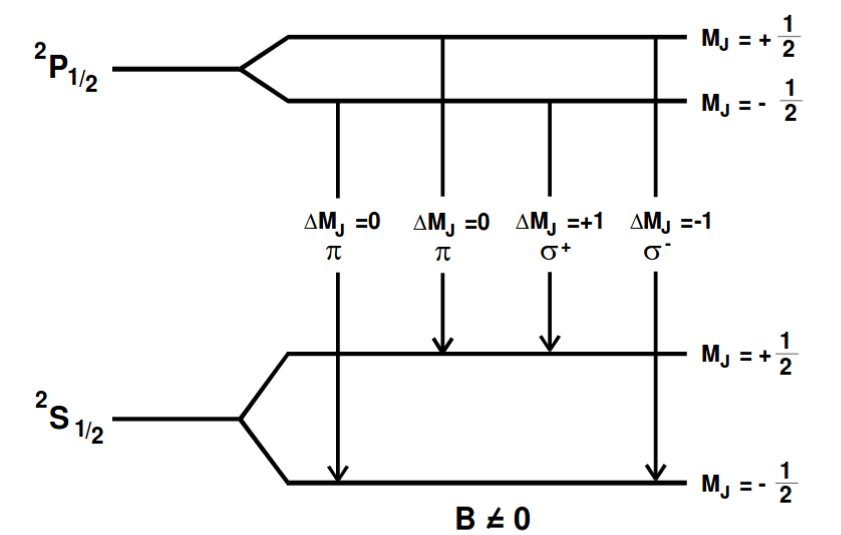
\includegraphics[height=6cm]{ressources/theorie1.png}
  \caption{Beispiel von möglichen Strahlungsübergängen zwischen verschiednen Anregungen eines Alkali-Atoms in einem äußeren Magnetfeld \cite{skript}.}
  \label{fig:theorie}
\end{figure}

In hier besprochenen Beispiel existieren die beiden Zustände $^2 \text{P}_{\sfrac{1}{2}}$ und $ ^2 \text{S}_{\sfrac{1}{2}}$ \footnote{Es wird die spektroskopische Notation $^{2S+1} L_J$ verwendet.}, wobei die Zustände aufgrund eines äußeren Magnetfeldes jeweils in $M_J = \pm \sfrac{1}{2}$ aufgespalten sind.
Es existieren verschiedene Strahlungsübergänge zwischen den Niveaus, welche durch Energie sowie Polarisation gekennzeichnet sind.
Beim $\sigma^+$-Übergang lautet die Auswahlregel $\Delta M_J = + 1$ und die involvierten Lichtquanten sind rechts-polarisiert, während bei einem $\sigma^-$-Übergang $\Delta M_J = - 1$ gilt und Spin und Ausbreitungsrichtung der Lichtquanten parallel sind.
Zudem exisiteren sogenannte $\pi$-Übergänge, bei denen $\Delta M_J = 0$ ist und das Licht linear polarisiert ist.
Die Polarisationsrichtung ist hier parallel zu $\vec{B}$.
Im thermischen Gleichgewicht ist im hier betrachteten System laut Gleichung \eqref{eqn:1} der energetisch niedrigste Zustand, hier $^2 \text{S}_{\sfrac{1}{2}}, \Delta M_J = -\sfrac{1}{2}$ am stärksten besetzt.
Das optische Pumpen besteht nun darin, die Atome mit rechtszirkular-polarisierten $D_1$-Licht zu bestrahlen, so dass $\sigma^-$-Übergänge induziert werden.
Hierdurch wird der Zustand $^2 \text{P}_{\sfrac{1}{2}}, \Delta M_J = + \sfrac{1}{2}$ besetzt.
Von dort findet spontane Emission statt, so dass der angeregte Zustand bereits nach kurzer Zeit wieder in einem der beiden $ ^2 \text{S}_{\sfrac{1}{2}}$-Zustände übergeht.
Da die $\sigma^-$ Anregung jedoch nicht dazu in der Lage ist, die Atome im $M_J = + \sfrac{1}{2}$-Zustand wieder anzuregen und auch kein direkter Übergang zwischen den beiden Grundzuständen möglich ist, findet eine Ansammlung im energetisch höheren Grundzustand statt.
Diese Inversion kann experimentell daran beobachtet werden, dass die Transparenz der Zelle, in dem sich die Atome befinden, zunimmt:
Bevor das optische Pumpen erfolgt ist, wurde das zirkular-polarisierte Licht absorbiert.
Nach der Inversion findet dieser Absorption nicht mehr statt, so dass der Verlauf der Transparenz, dargestellt in Abbildung \ref{fig:theorie2}, ein Indiz für das erfolgreiche optische Pumpen ist.

\begin{figure}
  \centering
  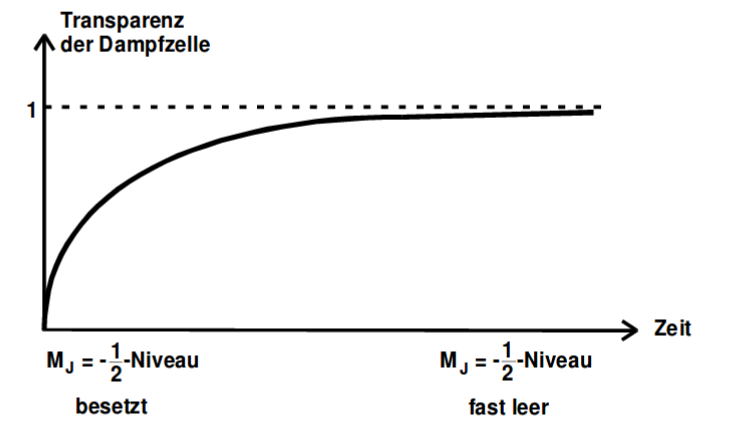
\includegraphics[height=6cm]{ressources/theorie2.png}
  \caption{Verlauf der Transparenz der Zelle durch optisches Pumpen \cite{skript}.}
  \label{fig:theorie2}
\end{figure}



%\cite{sample}

% 2x2 Plot
% \begin{figure*}
%     \centering
%     \begin{subfigure}[b]{0.475\textwidth}
%         \centering
%         \includegraphics[width=\textwidth]{Abbildungen/Schaltung1.pdf}
%         \caption[]%
%         {{\small Schaltung 1.}}
%         \label{fig:Schaltung1}
%     \end{subfigure}
%     \hfill
%     \begin{subfigure}[b]{0.475\textwidth}
%         \centering
%         \includegraphics[width=\textwidth]{Abbildungen/Schaltung2.pdf}
%         \caption[]%
%         {{\small Schaltung 2.}}
%         \label{fig:Schaltung2}
%     \end{subfigure}
%     \vskip\baselineskip
%     \begin{subfigure}[b]{0.475\textwidth}
%         \centering
%         \includegraphics[width=\textwidth]{Abbildungen/Schaltung4.pdf}    % Zahlen vertauscht ... -.-
%         \caption[]%
%         {{\small Schaltung 3.}}
%         \label{fig:Schaltung3}
%     \end{subfigure}
%     \quad
%     \begin{subfigure}[b]{0.475\textwidth}
%         \centering
%         \includegraphics[width=\textwidth]{Abbildungen/Schaltung3.pdf}
%         \caption[]%
%         {{\small Schaltung 4.}}
%         \label{fig:Schaltung4}
%     \end{subfigure}
%     \caption[]
%     {Ersatzschaltbilder der verschiedenen Teilaufgaben.}
%     \label{fig:Schaltungen}
% \end{figure*}
